\chapter{SpringBoot~项目}
\section{整体概述}
本部分是使用SpringBoot重构整个项目的后端部分。目的是提供一套完整正确的用户点餐后端程序,和一套完备的可拓展可维护的后端结构。

\section{项目技术架构}
JDK17 MySQL SpringBoot Maven3.6.3

\section{设计}

\subsection{模块设计}
四个阶段的项目加上组内实现的创新和优化,代码共计四万余行,为了应对庞大的工程量以及确保项目的可维护性与可拓展性,我们采用了模块化设计的方法。各个模块被设计为相对独立的单元,为了满足高内聚低耦合的特性。在模块划分上,整个项目沿用了~SpringBoot~框架的分层架构,按照以下的方式组织。
\begin{figure}[htbp]
    \centering
    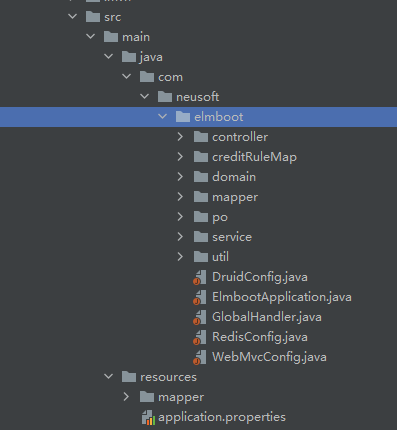
\includegraphics[width=0.8\textwidth]{elm_springboot_framework}
    \caption{项目结构模块设计}\label{fig:elm_springboot_framework}
    \vspace{\baselineskip}
\end{figure}

\subsubsection{表现层~(Presentation Layer)~}
表示层通常负责应用程序的用户界面部分,用于与用户进行交互和处理用户用户请求。它通常包括控制器~(Controller)~或路由~(Router)~层,这些组件接收来自前端或其他客户端的请求,并将它们路由到适当的处理程序。在本项目中,表示层由前端项目负责实现,后端只负责提供接口。在前端项目中,我们使用~Vue3~框架,主要的内容和部分都在上文已有介绍,在这里不做赘述。

\subsubsection{业务层~(Service Layer)~}
业务层是整个模块的核心部分,负责处理业务逻辑和业务规则。在本项目中,业务层由~SpringBoot~项目负责实现。在业务层中,我们使用了~Spring~框架提供了依赖注入和事务管理等丰富的特性,可以有助于简化业务逻辑的编写和管理。

\subsubsection{持久层~(Persistence Layer)~}
持久层负责与后端数据存储进行交互,在本项目中,使用~Spring~框架提供的对于~MySQL~数据库的数据访问技术支持,如JDBC等。在这一层,本项目定义了数据访问对象~(Dao)~来执行数据库操作。

\subsubsection{模型层~(Module Layer)~}
模型层是应用程序的数据表示层。它包括实体~(Entry)~或~(POJO)~类,这些类通常用于表示应用程序中的数据结构。模型层的对象通常与数据库表之间崔在因施工和关系,这些由数据访问层负责管理。

\subsection{数据库设计}

\subsubsection{后台管理数据库设计}
由于阶段一要实现饿了么管理员对于每一个商家得管理,每个商家又要对自身的基本信息(例如起送费、配送费)进行管理。因此我们要有一张商家表以及管理员表。商家表的设计如表\ref{tab:table_6_1} 所示,管理员表的设计如表\ref{tab:table_6_2}所示。这里特别需要提出的是,由于起送费和配送费小数点后边不会超过两位,我们这里特地把~starPrice~和~deliveryPrice~字段的数据类型设置为~decimal~。

\begin{table}[htbp]
    \caption{商家列表}\label{tab:table_6_1}
    \vspace{0.5em}\wuhao
    \begin{tabularx}{\hsize}{@{\extracolsep{\fill}}c c c}
    \toprule[1.5pt]
    字段名          & 数据类型  & 说明 \\ 
    \midrule[1pt]
    businessId      & int      & 商家编号 \\
    password        & varchar  & 密码 \\
    businessName    & varchar  & 商家名称 \\
    businessAddress & varchar  & 商家地址 \\
    businessExplain & varchar  & 商家介绍 \\
    starPrice       & decimal  & 起送费 \\
    deliveryPrice   & decimal  & 配送费 \\
    \bottomrule[1.5pt]
    \end{tabularx}
\vspace{\baselineskip}
\end{table}

\begin{table}[htbp]
    \caption{管理员表}\label{tab:table_6_2}
    \vspace{0.5em}\wuhao
    \begin{tabularx}{\hsize}{@{\extracolsep{\fill}}c c c}
    \toprule[1.5pt]
    字段名          &  数据类型  &   说明 \\ 
    \midrule[1pt]
    adminId      & int     & 管理员编号 \\
    adminName   & varchar  & 管理员名称 \\
    password    & varchar  & 密码   \\

    \bottomrule[1.5pt]
    \end{tabularx}
\vspace{\baselineskip}
\end{table}

又由于每个商家要对自身出售的商品进行管理,因此我们需要一个食品表。食品表的设计如表\ref{tab:table_6_3} 所示。同样由于食品价格小数点后边不会超过两位,我们这里特地把~foodPrice~字段的数据设置为~decimal~。同时~businessId~字段为~buisiness~表的~businessId~字段的外键。

\begin{table}[htbp]
    \caption{食品表}\label{tab:table_6_3}
    \vspace{0.5em}\wuhao
    \begin{tabularx}{\hsize}{@{\extracolsep{\fill}}c c c}
    \toprule[1.5pt]
    字段名          &  数据类型  &   说明 \\ 
    \midrule[1pt]
    foodId      & int     & 食品编号 \\
    foodName   & varchar  & 食品名称 \\
    foodExplain    & varchar  & 食品介绍   \\
    foodPrice      & decimal     & 食品价格 \\
    businessId      & int     & 所属商家编号 \\
    \bottomrule[1.5pt]
    \end{tabularx}
\vspace{\baselineskip}
\end{table}

\subsubsection{点餐业务数据库设计}

点餐业务中需要记录每一个用户的信息,以便实现登录历史订单查询等功能,需要一个用户表来记录每一个用户的信息。用户表的设计如表\ref{tab:table_6_4} 所示。

\begin{table}[htbp]
    \caption{用户表}\label{tab:table_6_4}
    \vspace{0.5em}\wuhao
    \begin{tabularx}{\hsize}{@{\extracolsep{\fill}}c c c}
    \toprule[1.5pt]
    字段名          &  数据类型  &   说明 \\ 
    \midrule[1pt]
    userId      & varchar     & 食品编号 \\
    password   & varchar  & 食品名称 \\
    userName    & varchar  & 食品介绍   \\
    userSex      & int     & 食品价格 \\
    userImg      & mediumtext     & 所属商家编号 \\
    delTag      & int     & 所属商家编号 \\
    \bottomrule[1.5pt]
    \end{tabularx}
\vspace{\baselineskip}
\end{table}

点餐业务中需要向用户展示全部的商家信息,所以我们需要有一张商家表。每个商家又需要向顾客展示所售卖的全部食物,于是需要有一张食品表。其中食品表中的~businessId~字段是食品表中的~businessId~字段的外键。商家表的设计如表\ref{tab:table_6_5},食品表的设计如表\ref{tab:table_6_6}所示。

\begin{table}[htbp]
    \caption{商家表(点餐业务)}\label{tab:table_6_5}
    \vspace{0.5em}\wuhao
    \begin{tabularx}{\hsize}{@{\extracolsep{\fill}}c c c}
    \toprule[1.5pt]
    字段名          &  数据类型  &   说明 \\ 
    \midrule[1pt]
    businessId   & int  & 商家编号 \\
    businessName    & varchar  & 商家名称   \\
    businessAddress  & varchar & 商家地址 \\
    businessExplain     & varchar     & 商家介绍 \\
    businessImg      & mediumtext     & 商家图片 \\
    orderTypeId      & int     & 共用10种点餐分类 \\
    starPrice      & decimal     & 起送费 \\
    deliveryPrice      & decimal     & 配送费 \\
    remarks     & varchar     & 备注 \\
    \bottomrule[1.5pt]
    \end{tabularx}
\vspace{\baselineskip}
\end{table}

\begin{table}[htbp]
    \caption{食品表(点餐业务)}\label{tab:table_6_6}
    \vspace{0.5em}\wuhao
    \begin{tabularx}{\hsize}{@{\extracolsep{\fill}}c c c}
    \toprule[1.5pt]
    字段名          &  数据类型  &   说明 \\ 
    \midrule[1pt]
    foodId      & int     & 食品编号 \\
    foodName   & varchar  & 食品名称 \\
    foodExplain    & varchar  & 食品介绍   \\
    foodImg      & mediumtext     & 食品图片 \\
    foodPrice      & decimal     & 食品价格 \\
    businessId      & int     & 所属商家编号 \\
    businessId      & varchar     & 备注 \\
    \bottomrule[1.5pt]
    \end{tabularx}
\vspace{\baselineskip}
\end{table}

又由于要实现用户能够选购商品的功能,需要有一个购物车表来记录用户在特定商家所选购的商品。购物车表中的~foodId~字段为食品表中~foodId~字段的外键,~businessId~字段为商家表中~businessId~的外键,~userId~字段为用户表中~userId~字段的外键。购物车表的设计如表\ref{tab:table_6_7}所示。

\begin{table}[htbp]
    \caption{购物车表}\label{tab:table_6_7}
    \vspace{0.5em}\wuhao
    \begin{tabularx}{\hsize}{@{\extracolsep{\fill}}c c c}
    \toprule[1.5pt]
    字段名          &  数据类型  &   说明 \\ 
    \midrule[1pt]
    cardId      & int     & 无意义编号 \\
    foodId   & int  & 食品名称 \\
    businessId    & int  & 所属商家编号   \\
    userId      & varchar     & 所属用户编号 \\
    quantity      & int     & 同一类型食品的购买数量 \\
    \bottomrule[1.5pt]
    \end{tabularx}
\vspace{\baselineskip}
\end{table}

每一个用户都有不同的送货地址,所以我们需要一个送货地址表来记录每
一个用户所对应的配送地址,送货地址表中的~userId~字段为用户表中的~userId~字
段的外键。送货地址表的设计如表\ref{tab:table_6_8}所示。

\begin{table}[htbp]
    \caption{送货地址表}\label{tab:table_6_8}
    \vspace{0.5em}\wuhao
    \begin{tabularx}{\hsize}{@{\extracolsep{\fill}}c c c}
    \toprule[1.5pt]
    字段名          &  数据类型  &   说明 \\ 
    \midrule[1pt]
    daId      & int     & 送货地址编号 \\
    contactName   & varchar  & 联系人姓名 \\
    contactSex    & int  & 联系人性别   \\
    contactTel   & varchar     & 联系人电话 \\
    address      & varchar     & 送货地址 \\
    userId      & varchar     & 所属用户编号 \\
    \bottomrule[1.5pt]
    \end{tabularx}
\vspace{\baselineskip}
\end{table}

用户选购完商品之后,需要能够进行对购物车中所选购的商品进行下单,这就需要一个订单表和一个订单明细表。订单表中的~userId~字段为用户表中的~userId~字段的外键,~businessId~字段为商家表中~businessId~字段的外键,~daId~字段为送货地址表中~daId~字段的外键。订单明细表中的~orderId~字段为订单表中的~orderId~字段的外键,~foodId~字段为食品表中~foodId~字段的外键。订单表的具体实现如表\ref{tab:table_6_9}所示,~订单明细表的具体实现如表\ref{tab:table_6_10}所示。

\begin{table}[htbp]
    \caption{订单表}\label{tab:table_6_9}
    \vspace{0.5em}\wuhao
    \begin{tabularx}{\hsize}{@{\extracolsep{\fill}}c c c}
    \toprule[1.5pt]
    字段名          &  数据类型  &   说明 \\ 
    \midrule[1pt]
    orderId      & int     & 订单编号 \\
    userId   & varchar  & 所属用户编号 \\
    businessId    & int  & 所属商家编号   \\
    orderDate   & varchar     & 订购日期 \\
    orderTotal      & decimal     & 订单总价 \\
    daId      & int     & 所属送货地址编号 \\
    orderState      & int     & 订单状态(0未支付,1已支付) \\
    \bottomrule[1.5pt]
    \end{tabularx}
\vspace{\baselineskip}
\end{table}

\begin{table}[htbp]
    \caption{订单明细表}\label{tab:table_6_10}
    \vspace{0.5em}\wuhao
    \begin{tabularx}{\hsize}{@{\extracolsep{\fill}}c c c}
    \toprule[1.5pt]
    字段名          &  数据类型  &   说明 \\ 
    \midrule[1pt]
    odId      & int     & 订单明细编号 \\
    orderId   & int  & 所属订单编号 \\
    foodId    & int  & 所属食品编号   \\
    quantity   & int     & 数量 \\
    \bottomrule[1.5pt]
    \end{tabularx}
\vspace{\baselineskip}
\end{table}

\subsection{接口设计}

\subsubsection{外部接口}
用户或其他软件可以通过~Interne~访问服务器~IP~实现对本软件的访问。同时提供图形化UI界面供用户使用。并且提供其他软件能够访问本项目的接口。网络传输协议采用HTTP协议,具体使用方法为:~http://IP地址/数据库名/内部接口~

\subsubsection{内部接口}
内部接口主要是为了实现软件的功能,提供给前端调用。内部接口的具体实现如下所示。

接口的部分已经在第三部分Serverlet部分阐述过,这里不做赘述。


\section{点赞业务流后端的SpringBoot实现}
点餐业务流后端采用~SpringBoot+Mybatis~实现,利用~Mybatis~连接并操作数据库,使得对于数据库的操作代码编写简单。~SpringBoot~框架采用三层架构,即控制层、业务层和持久层。控制层向上层即前端提供接口,使得前端可以调用后端接口;业务层实现具体业务代码,如数据库的事务型操作在这里体现;持久层即编写~SQL~语句操作数据库,实现对数据库的修改和访问。三层架构中,除持久层外,其余层代码较为简单,大致模板如下,除部分业务代码外不再给出具体实现:

\begin{lstlisting}[basicstyle=\footnotesize]
//控制层代码模板
@RestController
@RequestMapping("/XXXXController")
public class XXXXController {
    
    @Autowired
    private XXXXService xxxxService;

    @RequestMapping("接口名/")
    public 返回值类型接口名参数类型( 参数名)throws Exception{
        return xxxxService接口名参数名.();
    }
    
    ...
}
\end{lstlisting}

\begin{lstlisting}[basicstyle=\footnotesize]
//业务层接口代码模板
public interface XXXXService {
    public 返回值类型接口名参数类型( 参数名);
    ...
}
\end{lstlisting}

\begin{lstlisting}[basicstyle=\footnotesize]
//业务层实现代码模板
@Service
public class XXXXServiceImpl implements XXXXService{
    @Autowired
    private XXXXMapper xxxxMapper;
    @Override
    public 返回值类型接口名参数类型( 参数名) {
        return xxxxMapper接口名参数名.();
    }
    ...
}
\end{lstlisting}

其中,“XXXX”为对应的类,详见图\ref{fig:table_forSB}.
点餐业务流共涉及对客户表、地址表、商家表、食品表、购物车表、订单
表和订单明细表的修改与访问,具体如下。

\begin{figure}[htbp]
    \centering
    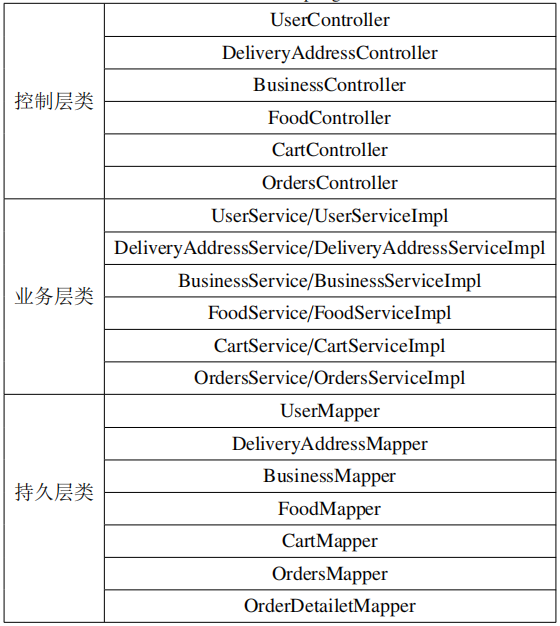
\includegraphics[width=0.8\textwidth]{table_forSB}
    \caption{点餐业务流SpringBoot实现类}\label{fig:table_forSB}
    \vspace{\baselineskip}
\end{figure}

\section{用户信息模块功能实现}
本模块,涉及对用户表和地址表的修改与访问。~SQL~语句较为简单、因此采用注解的方式直接写在~Java~代码中。

\begin{lstlisting}[basicstyle=\footnotesize]
//对表的修改与查询User
@Mapper
public interface UserMapper {
    @Select("select * from user where userId=#{userId} and
        password=#{password}")
    public User getUserByIdByPass(User user);
    @Select("select count(*) from user where userId=#{userId}")
    public int getUserById(String userId);
    @Insert("insert into user
        values(#{userId},#{password},#{userName},#{userSex},null,1)")
    public int saveUser(User user);
}
\end{lstlisting}


\begin{lstlisting}[basicstyle=\footnotesize]
//对地址表的修改与查询
@Mapper
public interface DeliveryAddressMapper {
    @Select("select * from deliveryAddress where userId=#{userId} 
        order by daId")
    public List<DeliveryAddress> listDeliveryAddressByUserId(String
        userId);
    @Select("select * from deliveryAddress where daId=#{daId}")
    public DeliveryAddress getDeliveryAddressById(Integer daId);
    @Insert("insert into deliveryAddressvalues(null,#{contactName},
        #{contactSex},#{contactTel},#{address},#{userId})")
    public int saveDeliveryAddress(DeliveryAddress deliveryAddress);
    @Update("update deliveryAddress set contactName=#{contactName}
        ,contactSex=#{contactSex},contactTel=#{contactTel},
        address=#{address}where daId=#{daId}")
    public int updateDeliveryAddress(DeliveryAddress 
        deliveryAddress);
    @Delete("delete from deliveryAddress where daId=#{daId}")
    public int removeDeliveryAddress(Integer daId);
}
\end{lstlisting}

\section{商家信息模块}
本模块涉及对商家表和食品表的修改与访问。简单的 SQL 语句不再给出实现,部分较为复杂的 SQL 语句写在 XML 文件中,如模糊查询、参数不定等。

\begin{lstlisting}[basicstyle=\footnotesize]
SELECT * FROM (
    SELECT COUNT(o.orderId)
        num,b.businessId,b.businessAddress,b.businessExplain,
        b.businessImg,b.businessName,b.deliveryPrice,
        b.orderTypeId,b.remarks,b.starPrice,o.orderId
    FROM business b LEFT OUTER JOIN (
        SELECT orders.businessId,orders.orderId FROM orders WHERE
        orders.userId=#{userId}
    ) o
    ON o.businessId = b.businessId GROUP BY b.businessId) a
ORDER BY a.num DESC
\end{lstlisting}

\section{点单业务模块}
本模块涉及对购物车表、订单表和订单明细表的修改与访问。在创建订单时涉及到事务,即要么不执行,要么全部执行。在~SpringBoot~框架中使用注解
~“@Transactional”~说明某方法是一个事务。

\begin{lstlisting}[basicstyle=\footnotesize]
@Service
public class OrdersServiceImpl implements OrdersService{
    private CartMapper cartMapper;
    @Autowired
    private OrdersMapper ordersMapper;
    @Autowired
    private OrderDetailetMapper orderDetailetMapper;
    @Override
    @Transactional
    public int createOrders(Orders orders) {
        //查询当前用户购物车中当前商家的所有食品1.
        Cart cart = new Cart();
        cart.setUserId(orders.getUserId());
        cart.setBusinessId(orders.getBusinessId());
        List<Cart> cartList = cartMapper.listCart(cart);
        //创建订单(返回生成的订单编号)2.
        orders.setOrderDate(CommonUtil.getCurremntDate());
        ordersMapper.saveOrders(orders);
        int orderId = orders.getOrderId();
        //批量添加订单明细3.
        List<OrderDetailet> list = new ArrayList<>();
        for(Cart c : cartList) {
            OrderDetailet od = new OrderDetailet();
            od.setOrderId(orderId);
            od.setFoodId(c.getFoodId());
            od.setQuantity(c.getQuantity());
            list.add(od);
        }
        orderDetailetMapper.saveOrderDetailetBatch(list);
        //从购物车表中删除相关食品信息4.
        cartMapper.removeCart(cart);
        return orderId;
    }
}
\end{lstlisting}

此外,在访问订单是,涉及到多表查询,即订单表连接订单明细表,订单表用于连接到商家表,~XML~的实现如下:

\begin{lstlisting}[basicstyle=\footnotesize]
<resultMap type="com.kbz320.elmboot.po.Orders" id="ordersResultMap">
    <id column="orderId" property="orderId"/>
    <result column="userId" property="userId"/>
    <result column="businessId" property="businessId"/>
    ...
    <association property="business"
        javaType="com.kbz320.elmboot.po.Business"
        select="com.kbz320.elmboot.mapper.BusinessMapper.getBusinessById"column="businessId"/>
    <collection property="list"
        ofType="com.kbz320.elmboot.po.OrderDetailet"
        select="com.kbz320.elmboot.mapper.OrderDetailetMapper.listOrderDetailetByOrderId"column="orderId"/>
</resultMap>

<select id="getOrdersById" parameterType="java.lang.Integer"
    resultMap="ordersResultMap">
    select * from orders where orderId=#{orderId}
</select>

<select id="listOrdersByUserId" parameterType="java.lang.String"
    resultMap="ordersResultMap">
    select * from orders where userId=#{userId}
</select>
\end{lstlisting}

其中,"association"表示一对一连接,而"collection"表示一对多连接。
